% Chapter 2

\chapter{Background Theory} % Write in your own chapter title
\label{Chapter2}
\lhead{Chapter 2. \emph{Background Theory}} % Write in your own chapter title to set the page header


\section{Player Behavior}
When a user plays a game there can be a high number of action combinations that can be performed that affects the user and his surroundings. Interacting with objects or other players differently over a different time period. These user actions (user telemetry) are registered in the game and play a crucial role for many game genres to analyze and find player behaviors and how they are evolving over time. Online game genres like social online games or Free-to-Play (F2P), in \textit{Facebook} and \textit{Google Play}, drive their revenue by e.g. analyzing player behavior to create actionable knowledge to be able to offer players to buy certain in-game items and upgrades for real money~\citep{Kim:2008Tracking, Drachen:2011Evaluating, Fields:2011SocialGame, Seif:2013GameAnalytics}.

Games running online persistent worlds where a game continues even a user quits the game, use player behavior analysis e.g. for balancing gameplay, in-game economy and game design. Major commercial games have been using behavior analysis for many years to help game design, Massively Multi-Player Online Role Play Games (MMORPG) play a special interests where the goal is to increase engagement of players playing the game in persistent worlds to have as many active monthly subscribers~\citep{Zoeller:2010, Yannakakis:2012}. 

F2P and Multi-Player Online (MMO) games allow large groups of players to interact in real-time, many of them in virtual worlds that are always running, allowing emergence of social communities in-game. These types of games can be highly driven by game metrics in game development, analyzing behaviors for e.g. customer acquisition and retention, evolving player communities and monetization~\citep{Drachen:2013GDM}.

\subsection{Game Player Metric}
When a user is playing a game he can e.g. interact with many items and other users, move through the game environment and purchase items. These kind of user actions is called user telemetry in context of collecting raw measurements data of user interactions in the game that is transmitted remotely to a game server where data about all users are stored and analyzed. 

Game player metrics are interpretable quantitative measures of one or more attributes from user telemetry, related either to revenue or players perspective~\citep{Drachen:2013Basics}. The revenue perspective player metric can be, e.g. Daily Active Users, Average Revenue Per User or when analyzing user attrition (churn) rate (a measure of the number of leaving users over a specific period of time). In players perspective, metrics are calculated related to user actions in-game, e.g. playtime of a user, average score, average hit/miss ratio, average puzzles solved. 

Game metrics can be variables (features) or more complex aggregates or calculated values. For example hit/miss ratio can be calculated by aggregating actions of a user when firing a weapon by sum multiple attributes like ``number of hits'' and ``number of misses'' to calculate the hit/miss ratio feature. Also calculating a metric as function of time, e.g. using the features ``player id'', ``session length'' and ``monsters killed'' to calculate the metric ``monsters killed per minute'' for each player \citep{Drachen:2013Basics}.

An example of a feature selection in a work by Drachen et al.~\citep{Drachen:2012}, analyzing user behavior telemetry in a major commercial title called \textit{Battlefield 2: Bad Company}, a first-person shooter game strategic and tactical elements. Of over 100 features to choose from the authors carefully selected 11 features to allow for evaluating the most important gameplay mechanics~\citep{Drachen:2009Tomb}, relating to character performance, game features and playtime. Some of the features selected were:
\begin{itemize}
\item \textbf{Score:} Number of points scored in total.
\item \textbf{Skill level:} Aggregated value of player skill.
\item \textbf{Total playtime:} Sum of player's time in total.
\item \textbf{Kill/Death ratio:} Number of kills the player has scored divided with number of his deaths.
\item \textbf{Score per minute:} Average score per minute of play.
\end{itemize}

A sub-category of player metrics called \textit{gameplay metrics}, measures of all in-game player behavior and interactions, e.g. navigation, using items and abilities, trading, using the game interface buttons and even the system/objects responses to player actions. Customer metric is another sub-category of the player metrics that usually receives higher priority considering the revenue chain in game development where it covers aspects of the user as a customer, e.g. virtual item purchases and other interactions with the game company, metrics that are interesting to marketing and the management~\citep{Drachen:2013Basics}. See Figure~\ref{fig:gamemetrics} showing a game metrics diagram with focus on the player metrics hierarchically structure.

Gameplay metrics are however the most important player metric when evaluating player experience, game designs and quality assurance~\citep{Kim:2008Tracking, Drachen:2012, Drachen:2011Evaluating}, but are generally in low priority compared to the customer metrics~\citep{Drachen:2013Basics}.
\begin{figure}[here]
\centerline{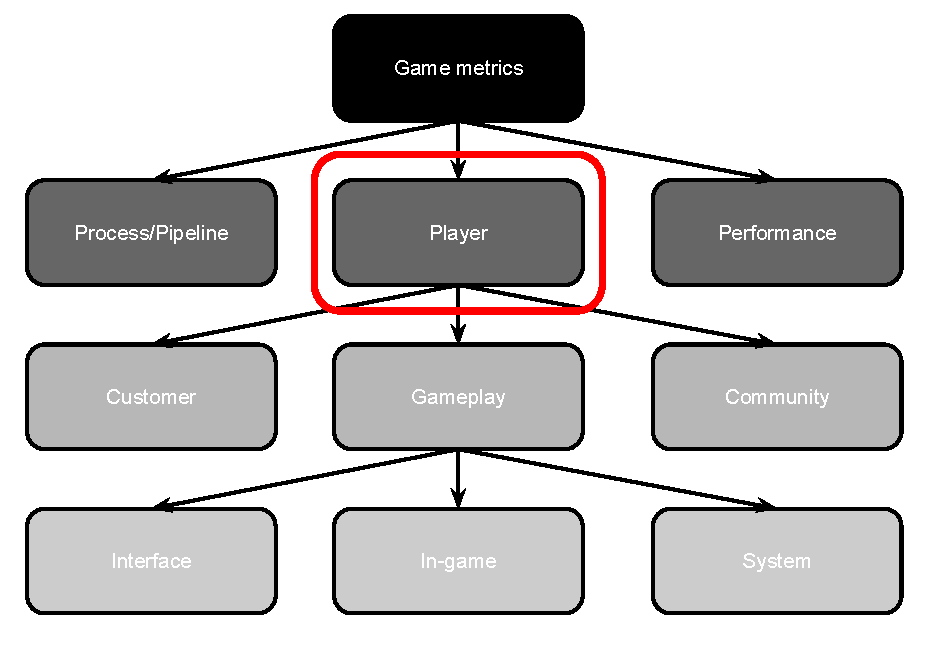
\includegraphics[width=0.9\textwidth]{Figures/Hierarchical_diagram_gamemetrics.pdf}}
\caption{Player metrics hierarchical diagram, Drachen et al. \textit{Game~Analytics - The Basics}~\citep{Drachen:2013Basics}. }
\label{fig:gamemetrics}
\end{figure}
There are huge amount of player behavior measures that are being logged each second in a complex game like MMORPG~\citep{Kim:2008Tracking, Drachen:2011Evaluating}, e.g. location of player, current health, stamina, status on weapons and a many more attributes that could describe a user state in a game also state/reactions of objects and monsters affected by the user. Its clear that this can generate a lot of information and game analysts face the problem of selecting the most essential pieces of information to analyze, imposing a bias but is necessary to avoid information overload~\citep{Drachen:2013Basics}. 

\section{Clustering}
The goal of clustering is to categories or groups similar objects (players, items, behaviors or any observations) together into so called clusters (hidden data structures) while different objects belong to other clusters. A cluster is a set of objects that are similar to each other while objects in different clusters are dissimilar to each other, having high intra-cluster similarity and low inter-cluster similarity~\citep{Xu:2009Clu}. Identifying descriptive features of an object one can compare these features to a known object based on their similarity or dissimilarity based on some criteria. Cluster analysis can be achieved by various algorithms and is a common technique in statistical data analysis that is used in many fields, e.g. machine learning, pattern recognition, image analysis and bioinformatics. The main purposes of clustering has been used for following purposes
\begin{itemize}
\item Gaining insights into data, anomaly (outlier) detection and finding the most important describing features in the underlying structure.
\item Identify the degree of similarity between objects, like natural classification.
\item Compressing or organizing the data and summarize through cluster prototypes.
\end{itemize}

In this thesis we focus on a popular clustering algorithm called k-means that is a centroid based clustering algorithm where a cluster prototype is represented by a central vector containing average value of all the objects in a cluster, e.g. describing the average behavior.

\subsection{K-means clustering method}
Many clustering methods exists but one of the most popular ones is called \textit{k-means}~\citep{FORGYE.W.:1965,MacQueen:1967KMeans}, also known as the Lloyd algorithm~\citep{Lloyd:1982} which was further generalized for vector quantization~\citep{Linde:1980VQ,Gersho:1991VQS,Xu:2009Clu}. K-means seeks to group similar data points into \textit{k} partitions or hyperspherical clusters giving insights into the general distributions in the dataset. A cluster is represented by a centroid that characterize the geometric center of the cluster that is calculated as the mean of all data instances belonging to that cluster. The objective function in k-means is to minimizes the squared error between a cluster's centroid (mean) and its assigned points and over all set of clusters minimizing the Sum of Squared Error (SSE). Let a set of data points $x_i \in \Re^d, i=1,...,N$, where each point $x$ is a real number $d$-dimensional vector and we want to partition them into \textit{K} clusters $C=\{c_1,...,c_K\} \in \Re^d$, then the objective function is defined as

\begin{center}
$SSE =\displaystyle \sum_{k=1}^{K}\displaystyle \sum_{x_i \in c_k}\left \| x_i-\mu_k \right \|^2$ 
\end{center}

where $\mu_k$ is the mean vector for the cluster centroid $k$ and $\left \| x_i-\mu_k \right \|$ is a Euclidean distance measure between two points the data vector $x_i$ and the mean vector $\mu_k$, calculated respectively

\begin{center}
$\mu_k = \dfrac{1}{N_k}\displaystyle \sum_{x_i \in c_k}x_i,$ 
\end{center}

where $c_k$ is a cluster number $k$ and its $N_k$ data points $i=1,...,N_k$. The Euclidean distance function is defined as

\begin{center}
$\left \| x_i-y_i \right \| = \sqrt{\displaystyle \sum_{i=1}^{d}(x_i-y_i)^2} $
\end{center}

When running the k-means algorithm it starts by initializing $K$ centroids by choosing random data points from the dataset or according some heuristic procedure. In each iteration of the algorithm it assigns data points to it's nearest centroid by calculating the minimum Euclidean distance to the $K$ centroids for each instance. After assigning all the data points to clusters the centroids are updated so they represent the mean value of all the points in the corresponding cluster. The algorithm stops the iteration when the centroids do not change from the previous iteration or the error (SSE) is below some specific threshold. Also possible to manually define a maximum number of iterations to be run. Algorithm~\ref{alg:km} shows a pseudo-code of k-means. The algorithm can be seen as a gradient descent procedure which iteratively updates its initial cluster centers so as to decrease its error function.
\algsetup{indent=2em}
\begin{center}
\newcommand{\km}{\ensuremath{\mbox{\sc K-means}}}
\begin{algorithm}[h!]
\caption{$\km(S,K)$}\label{alg:km}
\begin{algorithmic}[1]
\REQUIRE data set of instances $S = {x_i,...,x_n}$. $K$ number of clusters.  
\ENSURE $K$ clusters
\medskip
\STATE{Initialize K cluster centers}

\WHILE{termination condition is not satisfied} 
\STATE{Assign instances to the closest cluster center}
\STATE{Update cluster centers based on the assignments}
\ENDWHILE
\end{algorithmic}
\end{algorithm}
\end{center}
One of the weaknesses of k-means is that it is sensitive of the initial selection of the centroids which can lead to local optimum, that is the algorithm converges and fails to find the global optimum. One solution is to run the algorithm $n$ times and pick the initialization that gave the lowest SSE result. Another weakness of k-means is that a user has to predefine the number of centers k-means need to cluster, this is most often not known in advance. Many methods exist and most popular one is to run the algorithm with by increasing the $k$ number of clusters to some $K$ and pick a good $k$ candidate where the \textit{``elbow''} starts in the curve in a Scree plot \citep{Han:2006DM}. Noise in data and outliers can dramatically increase the squared error and centroids shifting from data distribution in question towards outliers far away, thus representing skewed distributions. Solutions involve removing these noise in preprocessing or normalize the data with the zero mean normalization \citep{Xu:2005Clustering, Han:2006DM}.

\textit{TODO INSERT PICTURE, showing a example of local optimum.}
%Example about local optimum%
%For example imagine if the global optimum is three cluster centroids each representing three separate data distributions then the algorithm fails to find the global optimum %if it initializes two centroids in one distribution and the last centroid in between the other two distributions. The algorithm stops and converges to local optimum.

The solution to the optimal partition can be found by checking all possibilities using a brute force method but that is a $NP$-hard problem \cite{Aloise:2009KmeansNPHard} and cannot be solved in a reasonable time. The k-means algorithm is a heuristic approach for the clustering problem with running time of the algorithm $O(NKdT)$ where $N$ is number data examples in $d$-dimensional space and $T$ is the number of iterations. Usually $K,d$ and $T$ is much less than $N$ meaning that k-means is good for clustering large-scale data because of approximately linear time complexity. The most computational work in k-means is the calculation of distances between objects and the cluster centers, in each iteration would require $O(Nk)$ distance computations. Calculating distances for each object is independent of each other, therefore these computations can be parallel executed.

The above implementation of k-means is called the \textit{batch} k-means, where the centroids are updated after all the data points have been assigned. The \textit{online} (incremental) mode of the algorithm processes each data point sequentially. For each data point $x$ the nearest cluster centroid $c_{min}$ is calculated and that centroid is updated right away, defined as 

\begin{center}
$c_{min}(old) = \underset{k}{\operatorname{argmin}} \|x-c_k\|$

$c_{min}(new) = c_{min}(old)+\eta(x-c_{min}(old))$
\end{center}

where the cluster centroid $c_{min}$ is updated towards the data point $x$ using the learning rate $\eta$ which determines the adaptation speed to each data point. The online approach is however highly dependent on the order of which the data points are processed. A variant of this method is used when clustering an endless stream of data where data points arrive one at a time or in chunks.


\subsection{Clustering Player Behaviors}
Cluster analysis in the context of game development is to find patterns of user behaviors, by reducing the dimensionality of the dataset in order to find the most important behavioral features and able to assign an expressive label to each found player profile. Behavioral clustering can answer questions like e.g. how people play the game, the average playing behavior, evolving behaviors, finding extreme archetypes and find clusters that describe unwanted behavior. Clustering player behaviors can give insights if a game is played as it is designed and obtain actionable knowledge that can be used to refine a game design~\citep{Drachen:2012}.

There are many clustering methods that can be applied to find player behaviors, the most popular ones in recent years finding interpretable behavior types (basis vectors or centroids) are \textit{k-means} and Simplex Volume Maximization (SIVM)~\citep{Drachen:2012, Drachen:2013}. Both clustering algorithms are applicable to large-scale data but are very different how they represent the behavior types. Figure~\ref{fig:SIVMvsKmeans} shows an example of how different basis vectors can be found using SIVM and k-means.
\begin{figure}[here]
\centerline{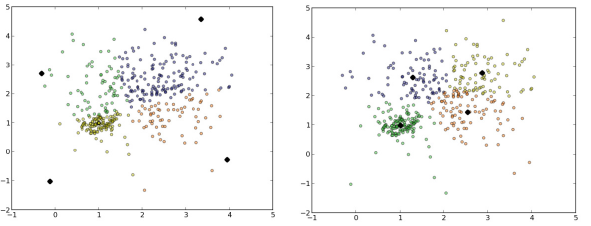
\includegraphics[width=0.9\textwidth]{Figures/SIVMvsKmeans.png}}
\caption{Simplex Volume Maximization (left picture) vs k-means. SIVM has four sparse basis vectors (black dots) and k-means has very similar centroids. The example is from a work of Drachen et al.~\citep{Drachen:2013}}
\label{fig:SIVMvsKmeans}
\end{figure}

SIVM is a Archetype Analysis (AA) approximation algorithm for large-scale data and its goal is to find the extreme (special) player behaviors whereas k-means focuses on the average player behaviors in compact clusters. Its easier to interpret the basis vectors from SIVM since they represent actual sparse data points where k-means cluster centroids (average of all data points in each cluster) can be very similar (in similar space) and more difficult to assign an expressive label. There are can be many challenges that need to be addressed when applying clustering algorithms to game behavior telemetry data e.g.
\begin{itemize}
\item The data can have a very high dimensionality, e.g. complex game interactions/mechanics from MMOGs.
\item The need to mix many different behavioral data types and use of normalization methods, e.g. numeric, categorical and bi-nominal.
\item Game telemetry data are often noisy and cleaning may be necessary, e.g. player pausing in a game, providing long play sessions.
\item The need for defining parameters for clustering, e.g. number of clusters for k-means.
\item Able to translate the findings to game developers, a knowledge that is actionable.
\end{itemize}

K-means algorithm has been shown to be very useful in behavioral analysis to obtain useful insights into in the general behaviors found in games, where AA like the SIVM algorithm can extract behavior player profiles based on the different distances to each of the extreme behaviors~\citep{Drachen:2013}. When choosing features for behavioral cluster analysis, Drachen et al.~\citep{Drachen:2009TGA, Drachen:2012} suggests that one should focus on features related to the core game mechanics and playtime. Interpreting basis vectors found by SIVM and k-means are illustrated in Figure~\ref{fig:sivmbasis} and Figure~\ref{fig:kmeansbasis}, where Drachen et al.~\citep{Drachen:2013}, in a very recent study, selected playtime and leveling speed as behavioral variables showing five leveling behaviors they found in the popular MMORPG game World of Warcraft.\\


\begin{figure}[here]
\centerline{\includegraphics[width=0.9\textwidth]{Figures/sivmbasis.png}}
\caption{Five SIVM basis vectors showing extreme leveling behaviors for Archetype Analysis. Each basis vector is an actual player and is a legal playing behavior thus very easy to interpret ~\citep{Drachen:2013}.}
\label{fig:sivmbasis}
\end{figure}


\begin{figure}[here]
\centerline{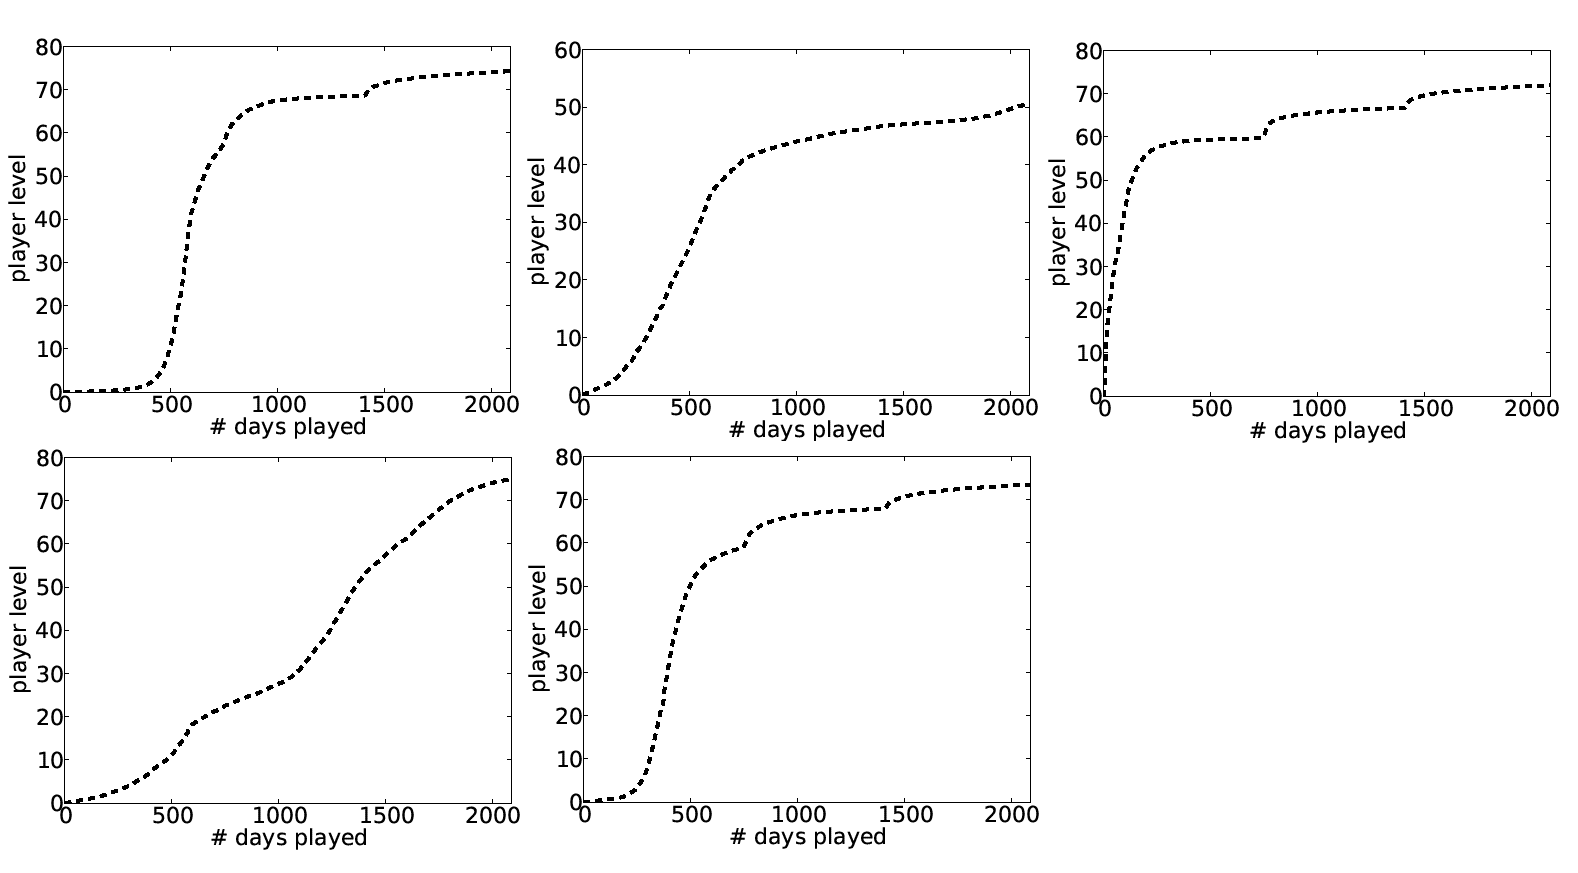
\includegraphics[width=0.9\textwidth]{Figures/kmeansbasis.png}}
\caption{K-means five cluster centroids showing average leveling behaviors representing each cluster of players. They give good idea about leveling behavior of many players but some of them are also very similar, interpretion is not straightforward~\citep{Drachen:2013}. }
\label{fig:kmeansbasis}
\end{figure}


\section{MapReduce and Large-Scale Data}
MapReduce is a programming model introduced by Google in 2004 \citep{Dean:2004}, built on the divide-and-conquer paradigm, dividing a large-scale data into smaller chunks and process them in parallel. MapReduce enables fault-tolerant distributed computing on large-scale datasets and is a new way to interact with \textit{Big Data} where as old techniques are more complicated, costly and time consuming \citep{Dean:2004, schneider2012Hadoop}. Google also introduced along with MapReduce a powerful distributed file system called \textit{Google File System} (GFS) that could hold massive amount of data. This led to a new open source software framework called Hadoop \citep{bialecki2005hadoop}, written in Java and is now maintained by Apache Foundation, a end-to-end solution for organizations that want to apply MapReduce. There are many Hadoop-related projects at Apache including the popular scalable machine learning and data mining library called Mahout, written also in Java. 

Hadoop builds on the MapReduce and GFS foundation, designed to abstract away much of the complexity of distributed processing running on large clusters of commodity computers. The MapReduce programming model allows developers to write parallel distributed programs very easily by only implementing two functions called \textit{Map} and \textit{Reduce}. Developers don't need to worry about doing a complicated code to e.g. distribute work to computers, internal communication, data transfers and dealing with fault tolerance. Instead they can focus on the logic to solve the problem at a hand.

\subsection{Programming Model}
As mentioned before a developer only needs to implement two functions Map and Reduce. The \textit{Map} function takes as input pair and produces an intermediate $(key,value)$ pair. The Map functions are run in parallel and produce many intermediate output pairs which is then grouped together with the same \textit{key} by the MapReduce framework and is passed along to the \textit{Reduce} function. The Reduce function receives a key and all of its set of values from all the Map functions, then it merges these values and typically produces zero or one output key and value pair per Reduce invocation.

\textbf{Example:} The problem of counting the number of occurrences of each word in a document, solved in MapReduce \citep{Dean:2004}. The Map function receives each word as input and emits the word as a key with count of 1, e.g. we have set of words $w_1,...,w_n$ in a document then the output from all Map functions would be the sequence of key value pairs: $(w_1,1),...,(w_n,1)$. See the pseudo-code for the Map function in Algorithm~\ref{alg:map}.
\algsetup{indent=2em}
\begin{center}
\newcommand{\map}{\ensuremath{\mbox{\sc Map}}}
\begin{algorithm}[h!]
\caption{$\map(key,value)$}\label{alg:map}
\begin{algorithmic}[1]
\REQUIRE key is document name, value is document contents.
\ENSURE $(key,value)$ pair: (word, occurrence of one).
\medskip
\FORALL{$word \in value$} \STATE{$EmitIntermediate(word,1)$}
\ENDFOR
\end{algorithmic}
\end{algorithm}
\end{center}
The MapReduce framework then groups and merges all the $(key,value)$ pairs from all the Map functions and invokes the Reduce function with input key as a word and list of all the Map counts as the values: $(w_i,[v_1,...,v_n])$ where $w_i$ is a specific word with $1,...,n$ counts of one, e.g. $(w_1, [1,1,1])$ if $w_1$ had three occurrences in the document. The reduce function will simply sum up all the counts and output a total count for each word, Algorithm~\ref{alg:reduce} shows the pseudo-code for Reduce.
\algsetup{indent=2em}
\begin{center}
\newcommand{\reduce}{\ensuremath{\mbox{\sc Reduce}}}
\begin{algorithm}[h!]
\caption{$\reduce(key,values)$}\label{alg:reduce}
\begin{algorithmic}[1]
\REQUIRE key is a word, values are list of occurrences for the word.
\ENSURE number of occurrences for a word.
\STATE $count \leftarrow 0$
\medskip
\FORALL{$value \in values$} \STATE{$count = count + value$}
\ENDFOR
\STATE $Emit(AsString(key, count))$
\end{algorithmic}
\end{algorithm}
\end{center}
The MapReduce also allows the developer to implement a \textit{Combiner} function to do a partial reducing task that is executed on the same computer node as the Map function, combining the intermediate values after execution of the Map function. In the example mentioned above if a Combiner is implemented it will receive the Map output $(w_1,1),...,(w_n,1)$ as input. The Combiner would then partly sum up the occurrences for each word (key) and output a intermediate sum for each word from the Map function. E.g. if $w_1$ had three occurrences then the output pair would be $(w_1,3)$ instead of $(w_1,1),(w_1,1),(w_1,1)$. The algorithm for a combine function can be found in Algorithm~\ref{alg:combine}, it can look exactly like the Reduce function we saw above since it is combining/reducing the information.
\algsetup{indent=2em}
\begin{center}
\newcommand{\combine}{\ensuremath{\mbox{\sc Combine}}}
\begin{algorithm}[h!]
\caption{$\combine(key,values)$}\label{alg:combine}
\begin{algorithmic}[1]
\REQUIRE Key pair from Map, where key is a word and value is a occurrences of one.
\ENSURE $(key,value)$ pair: (word, partly sum of occurrences).
\STATE $count \leftarrow 0$
\medskip
\FORALL{$value \in values$} \STATE{$count = count + value$}
\ENDFOR
\STATE $EmitIntermediate(key, count)$
\end{algorithmic}
\end{algorithm}
\end{center}
Using a Combiner reduces the information sent over the network to the Reduce functions by eliminating repetition of intermediate keys produced by the Map tasks. Input for the Reduce function is the same as before, a word and a list of all occurrences where they are now a partly sum values from all the Combiners, e.g. if $w_1$ has three occurrences from one Combiner and two occurrences from another, the input will be: $(w_1, [3,2])$, instead of $(w_1,[1,1,1,1,1])$ 

\subsection{MapReduce Hadoop Execution Flow}
When a user program calls the MapReduce program the following sequence of occurs. MapReduce splits the input data into $M$ pieces (typically 64MB) then starts up many copies of the user program on a cluster of machines. One of the copies is a \textit{Master controller}, the rest are workers which each get assigned a Map or a Reduce task from the master. The master keeps track of the $M$ Map and $R$ (user specified) Reduce tasks statuses, scheduling of tasks, re-executing work from failed workers and responsible for messaging and information flow between workers.

Each Map task is assigned one or more chunks of the input data and executes the Map function code written by the user. The Map task output is stored on a local disk in $R$ partitions, the master then notifies the Reduce task about the intermediate data. The Reduce task reads the data and sorts it by the intermediate keys, grouping all occurrences of the same key together. For each unique intermediate key encountered it passes the key and the corresponding occurrences to the Reduce function written by the user. Figure~\ref{fig:mapreduce} illustrates the execution flow that we just described, for more details one can look at work of Dean and Ghemawat ~\citep{Dean:2004} and Rajaraman and Ullman ~\citep{Rajaraman:2011MMD}.
\begin{figure}[here]
\centerline{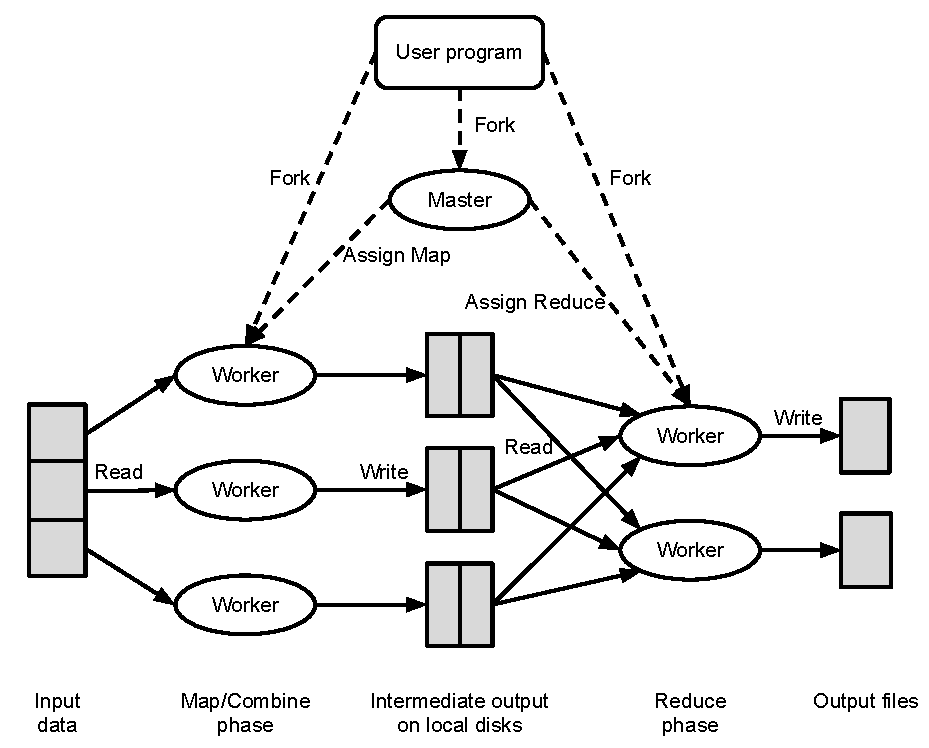
\includegraphics[width=0.9\textwidth]{Figures/MapReduceexecutionflow.pdf}}
\caption{Overview of the MapReduce execution flow}
\label{fig:mapreduce}
\end{figure}